\documentclass[11pt]{article} 
%\usepackage{amsbsy} % for \boldsymbol and \pmb 
%\usepackage{graphicx} % To include pdf files!
\usepackage{amsmath}
\usepackage{amsbsy}
\usepackage{amsfonts}
\usepackage{enumerate}
\usepackage[colorlinks=true, pdfstartview=FitV, linkcolor=blue, citecolor=blue, urlcolor=blue]{hyperref} % For links
\usepackage{fullpage}
\pagestyle{empty}
\usepackage{pgf,pgfplots,tikz}
\usepackage{amsmath,amssymb,amsthm}
\newcommand{\overrightharp}[1]{\hat{#1}}
\DeclareMathOperator{\proj}{proj}
\DeclareMathOperator{\years}{years}
\DeclareMathOperator{\cm}{cm}
\newcommand{\vct}{\mathbf}
\newcommand{\vctproj}[2][]{\proj_{{#1}}\vct{#2}}
\newtheorem{theorem}{Theorem}
\DeclareMathOperator{\m}{m}
\DeclareMathOperator{\kg}{kg}
\DeclareMathOperator{\N}{N}
\DeclareMathOperator{\Or}{or}
\DeclareMathOperator{\J}{J}
\DeclareMathOperator{\s}{s}
\DeclareMathOperator{\g}{g}
\DeclareMathOperator{\W}{W}
\DeclareMathOperator{\Heatoms}{He\hspace{1mm} atoms}
\DeclareMathOperator{\MeV}{MeV}
\DeclareMathOperator{\tr}{tr}
\newcommand{\norm}[1]{\left\lVert#1\right\rVert}
\usepackage{graphicx}
\newcommand{\abs}[1]{\lvert#1\rvert}
\DeclareMathOperator{\diverge}{div\,}
\DeclareMathOperator{\curl}{curl\,}
\title{\textbf{JCP221 Assignment}
\author{Maxim Piatine\\tut 9108}}
\date{}
\DeclareMathOperator{\lineint}{\int \mathbf{v}\cdot d\mathbf{l}}
\DeclareMathOperator{\surfint}{\int \mathbf{v}\cdot d\mathbf{a}}
\begin{document}
\maketitle
\section*{Question 1}
(a)Volume Calculation $V$:
\[V=0.8^3m^3=0.512m^3=512L\]
Moles Calculation $n$:
\[PV=nRT \Rightarrow \frac{PV}{RT}=n=\frac{(1atm)(512 L)}{(0.08206\frac{L\cdot atm}{K\cdot mol})(293K)}=21.3 mol\]
Ideal pressure at $505K$:
\[PV=nRT \Rightarrow P_{\text{ideal}}=\frac{nRT}{V}=\frac{(21.2946 mol)(0.08206 \frac{L\cdot atm}{K\cdot mol})(505 K)}{512L}=1.72atm\]
VDW pressure:
\[P=\frac{nRT}{V-nb}-a(\frac{n}{V})^2=\frac{(21.2946mol)(0.08206\frac{L\cdot atm}{K\cdot mol})(505K)}{512L-(21.2946mol\cdot  0.0366\frac{L}{mol})}-(1.33\frac{atm\cdot L^2}{mol^2})(\frac{(21.2946mol)}{512L})^2=1.72atm\]
(b)Surrounding calculation $\Delta S_{\text{sur}}$, no heat transfer ($q=0 \Rightarrow q_{\text{sur}}=-q=0$):
\[\Delta S_{\text{sur}}=\frac{q_{\text{sur}}}{T_{\text{sur}}}=0\]
$\Delta S$ Calculation:
\[\Delta S=nR\ln{\frac{V_2}{V_1}}+nC_{V,m}\ln{\frac{T_2}{T_1}}= 0+n(\frac{5}{2}R)\ln{\frac{T_2}{T_1}}=(21.2946mol)(\frac{5}{2})(8.315\frac{J}{K\cdot mol})\ln{\frac{505K}{293K}}=241\frac{J}{K}\]
Entropy total calculation $\Delta S_{\text{tot}}$:
\[\Delta S_{\text{tot}}=\Delta S+\Delta S_{\text{sur}}=(241\frac{J}{K})+0=241\frac{J}{K}\]
(c)Adiabatic irreversible process:
\[w=\Delta U=-P_{\text{ext}}\Delta V=-P_{\text{ext}}(V_2-V_1)\]
Diatomic Ideal Gas:
\[U=\frac{5}{2}nRT\]
\[U=\frac{5}{2}nR(T_2-T_1)\]
Ideal gas law:
\[PV=nRT \Rightarrow T=\frac{PV}{nR}\]
Substituting $T_2$ and $T_1$ with the ideal has law:
\[U=\frac{5}{2}nR(\frac{P_2V_2}{nR}-\frac{P_1V_2}{nR})=\frac{5}{2}(P_2V_2-P_1V_1)\]
Substituting $U$ into $w$ equation:
\[w=\frac{5}{2}(P_2V_2-P_1V_1)=-P_{\text{ext}}(V_2-V_1)\]
\[\frac{5}{2}P_2V_2-\frac{5}{2}P_1V_1=-P_{\text{ext}}V_2+P_{\text{ext}}V_1\]
\[\frac{5}{2}P_2V_2+P_{\text{ext}}V_2=P_{\text{ext}}V_1+\frac{5}{2}P_1V_1\]
\[V_2(\frac{5}{2}P_2+P_{\text{ext}})=P_{\text{ext}}V_1+\frac{5}{2}P_1V_1\]
\[V_2=\frac{P_{\text{ext}}V_1+\frac{5}{2}P_1V_1}{\frac{5}{2}P_2+P_{\text{ext}}}\]
(d)Using (c) calculate $V_2$ at $P_2=1.00$ atm and $T_2$:
\[V_2=\frac{(1.00 atm)(512L)+\frac{5}{2}(1.72 atm)(512 L)}{\frac{5}{2}(1.00 atm)+(1.00 atm)}=775L\]
Calculating $T_2$ using ideal gas law:
\[T_2=\frac{P_2V_2}{nR}=\frac{(1.00 mol)(775 L)}{(21.2946 mol)(0.08206 \frac{L\cdot atm}{K\cdot mol})}=444K\]
(e)Calculating $\Delta S_{\text{sur}}$, adiabatic process:
\[\Delta S_{\text{sur}}=\frac{q_{\text{sur}}}{T_{\text{sur}}}=0\]
Calculating $\Delta S$:
\[\Delta S=nR\ln{\frac{V_2}{V_1}+nC_{v,m}\ln{\frac{T_2}{T_1}}}\]
\[=(21.2946mol)(8.315 \frac{L\cdot atm}{K\cdot mol})\ln{\frac{775L}{512L}}+\frac{5}{2}(21.2946mol)(8.315 \frac{L\cdot atm}{K\cdot mol})\ln{\frac{444K}{505K}}=16.4 \frac{J}{K}\]
Calculating total entropy $\Delta S_{\text{tot}}$:
\[\Delta S_{\text{tot}}=\Delta S+\Delta S_{\text{sur}}=0+16.4\frac{J}{K}=16.4\frac{J}{K}\]
\newpage
(f) Enthalpy of oven:
\[\Delta H=\int^{T_2}_{T_1}C_P(T)dT\]
Since the temperature goes down from $505K$ to $293.15K$:
\[\int^{293.15K}_{505K}C_P(T)dT=\int^{293.15K}_{505K}(21.2946 mol)(8.315\frac{L\cdot atm}{K\cdot mol})(\frac{7}{2})dT=[619.726(\frac{L\cdot atm}{K})T |^{293.15K}_{505K}]\]
\[619.726(\frac{L\cdot atm}{K})(293.15K)-619.726(\frac{L\cdot atm}{K})(505K)=(181672L\cdot atm)-(312961L\cdot atm)=-1.31\cdot10^5J\]
Enthalpy of human:
\[\Delta H= 1.31\cdot10^5J\]
Heat Capacity of human:
\[\text{mass = molar mass }\cdot n \Rightarrow n=\frac{\text{mass}}{\text{molar mass}}=\frac{80kg}{18.02\frac{g}{mol}}=\frac{80000g}{18.02\frac{g}{mol}}=4439.51 mol\]
\[C_P=C_{P,m}\cdot n=(75.3 \frac{J}{\frac{K}{mol}})(4439.51mol)=3.34\cdot10^5\frac{J}{K}\]
Temperature change of human:
\[\Delta T=\frac{\Delta H}{C_P}=\frac{1.31\cdot10^5J}{3.34\cdot10^5\frac{J}{K}}=0.392K\]

\newpage
\section*{Question 2}
(a) The first graph shows a good linear agreement between the ideal gasses and Redlich-Kwong. The second graph shows a poor agreement.  
\begin{center}
    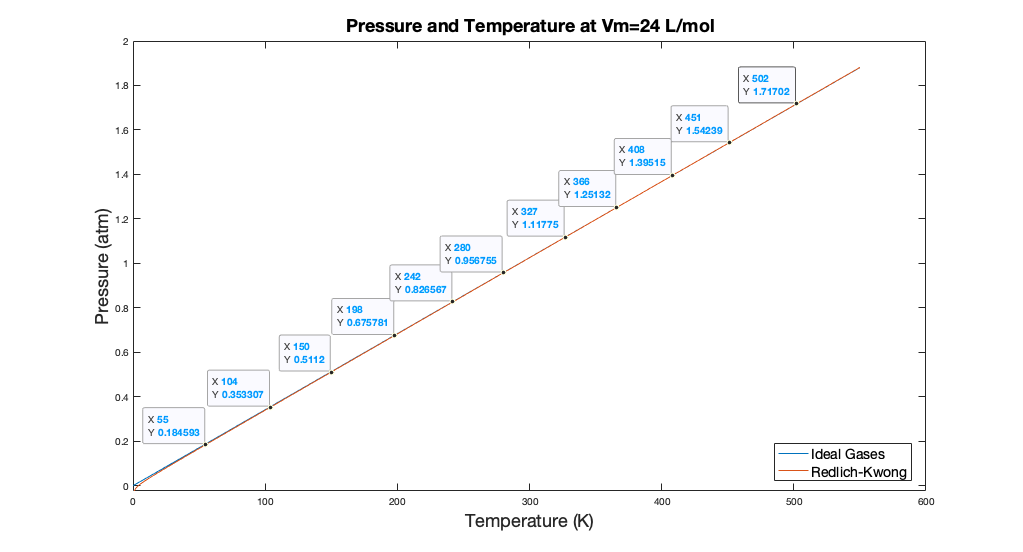
\includegraphics[width=15cm]{2.1.png}
\end{center}
\begin{center}
    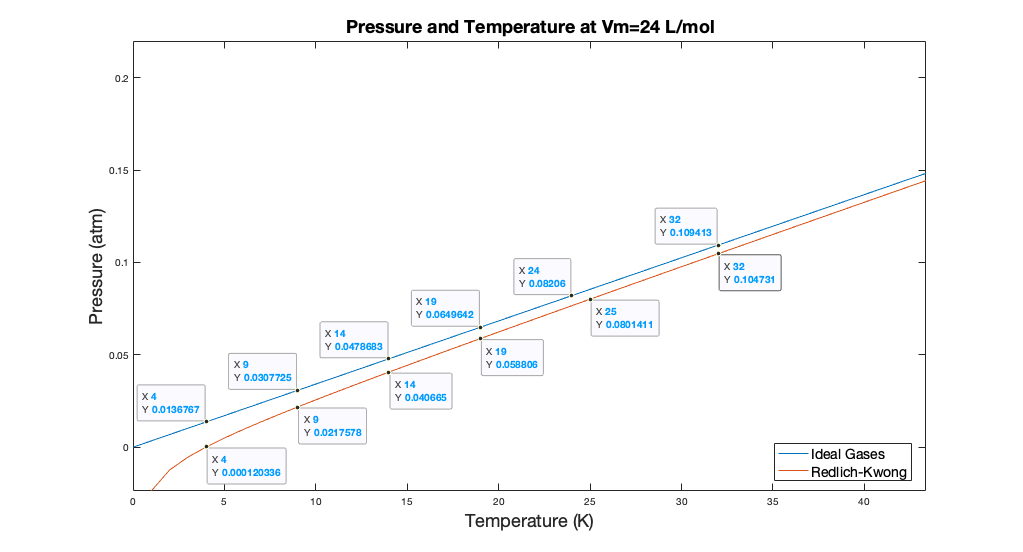
\includegraphics[width=15cm]{2.1.1.png}
\end{center}
\newpage
(b) The first graph shows a good linear agreement between the ideal gasses and Redlich-Kwong. The second graph shows a poor agreement.  
\begin{center}
    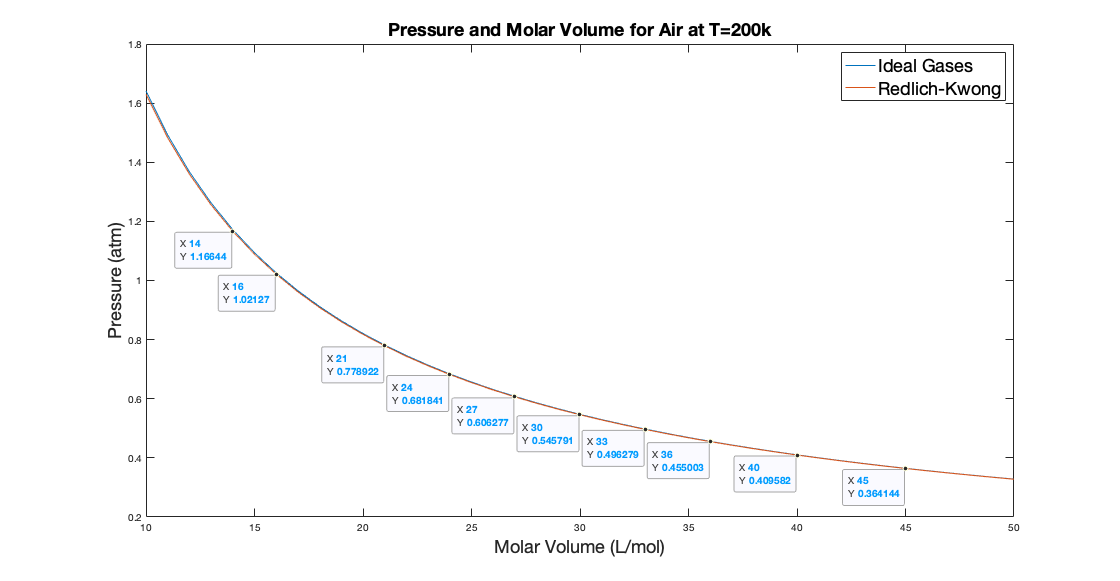
\includegraphics[width=15cm]{2.2.png}
\end{center}
\begin{center}
    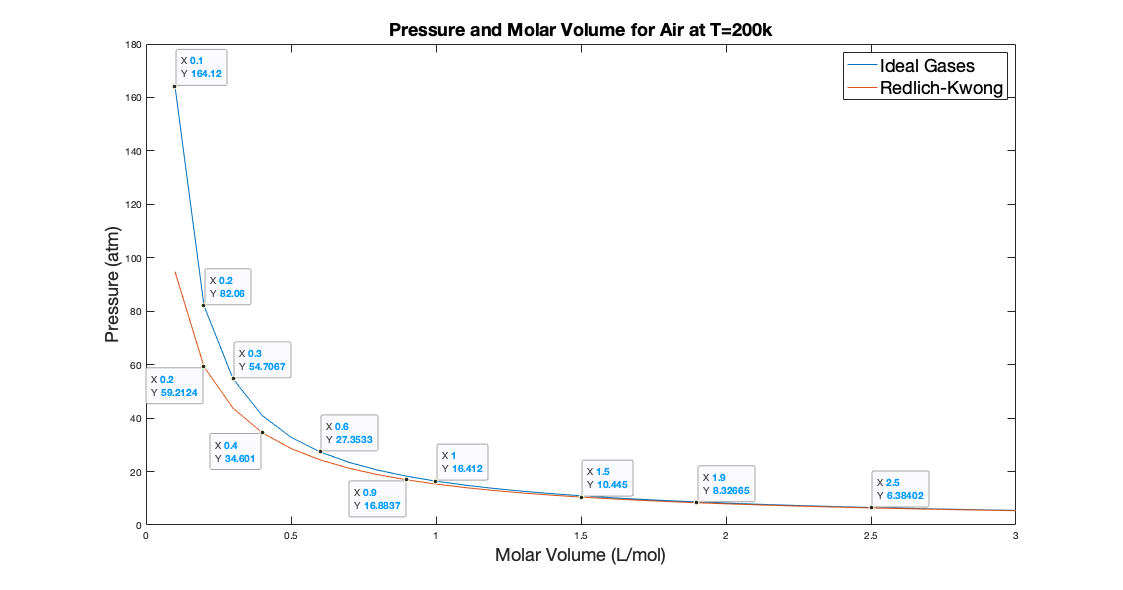
\includegraphics[width=15cm]{2.2.1.png}
\end{center}
\newpage
(c) Compression Factor vs Pressure:
\begin{center}
    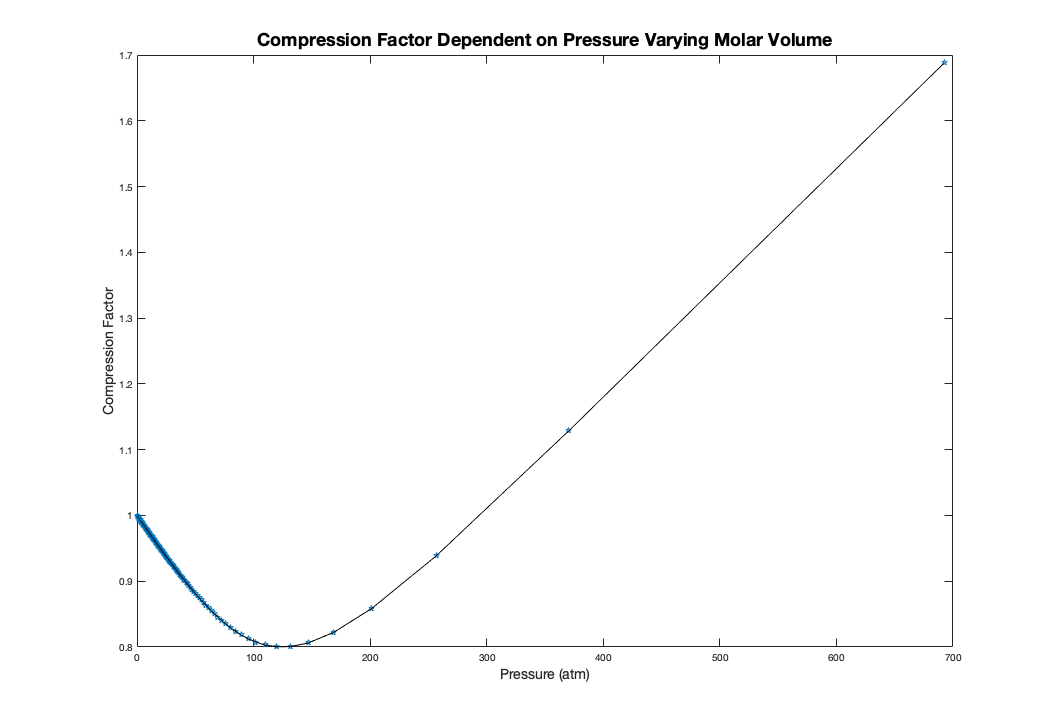
\includegraphics[width=17cm]{123.png}
\end{center}
\section*{Question 3}
(a) Point ($T_1,P_1$)=($444.6^\circ C, 1atm$)=($717.6 K, 101.3 kPa$). Using Clausius-Clapeyron equation:
\[P_2=P_1\exp{(-\frac{\Delta H^\circ}{R}[\frac{1}{T_2}-\frac{1}{T_1}])} \Rightarrow \ln{\frac{P_2}{P_1}}=-\frac{\Delta H^\circ}{R}[\frac{1}{T_2}-\frac{1}{T_1}] \Rightarrow -\frac{R}{\Delta H^\circ}\ln({\frac{P_2}{P_1}})=\frac{1}{T_2}-\frac{1}{T_1}\] 
\[-\frac{R}{\Delta H^\circ}\ln({\frac{P_2}{P_1}})+\frac{1}{T_1}=\frac{1}{T_2} \Rightarrow T_2=\frac{1}{-\frac{R}{\Delta H^\circ}\ln({\frac{P_2}{P_1}})+\frac{1}{T_1}}\]
Using $\Delta H^\circ= 277.2 \frac{kJ}{mol}$, $P_2=1.55 atm$, and $(T_1,P_1)$:
\[T_2=\frac{1}{-\frac{0.008315\frac{kJ}{K\cdot mol}}{277.2 \frac{kJ}{mol}}\ln({\frac{157.015kPa}{101.3kPa}})+\frac{1}{717.6K}}=724 K\]
(b) Point ($T_1,P_1$)=($95.31^\circ C, 5.1\cdot 10^{-6}atm$)=($368.46K,5.16\cdot 10^{-4} kPa$). Using Clausius-Clapeyron equation:
\[P_2=P_1\exp{(-\frac{\Delta H^\circ}{R}[\frac{1}{T_2}-\frac{1}{T_1}])}\]
Using $\Delta H^\circ= 279 \frac{kJ}{mol}$, $T_2=105.0^\circ C= 378.15K$, and $(T_1,P_1)$:
\[P_2=(5.16\cdot 10^{-4}kPa)\exp{(-\frac{279\frac{kJ}{mol}}{0.008315\frac{kJ}{K\cdot mol}}[\frac{1}{378.15K}-\frac{1}{368.46K}])}=5.32\cdot 10^{-3}kPa=5.25\cdot 10^{-5} atm\]
\newpage
\noindent (c) Point ($T_1,P_1$)=($95.31^\circ C, 5.1\cdot 10^{-6}atm$)=($368.46K,5.16\cdot 10^{-4} kPa$). Using Clausius-Clapeyron equation:
\[T_2=\frac{1}{-\frac{R}{\Delta H^\circ}\ln({\frac{P_2}{P_1}})+\frac{1}{T_1}}\]
Using $\Delta H^\circ= 279.14 \frac{kJ}{mol}$, $P_2=3.5\cdot10^{-6} atm= 3.55\cdot10^{-4}kPa$, and $(T_1,P_1)$:
\[T_2=\frac{1}{-\frac{0.008315\frac{kJ}{K\cdot mol}}{279.14\frac{kJ}{mol}}\ln({\frac{3.55\cdot10^{-4}kPa}{5.16\cdot10^{-4}kPa}})+\frac{1}{368.46K}}=367 K\]

\section*{Question 4}
Some thermodynamics practices that I deal with on a daily basis is related to cooking. When trying to cook pasta, for example, the process of boiling water is an isothermal process. If I have a lid on the container in which the water is boiling at a constant temperature causing the pressure to increases causing the volume to expand. There is some steam escaping the system and maybe causing the lid to shake making it an isothermal process. However, in this example it is non adiabatic since the heat from the system transfers to the outside and its surroundings. Making the process isothermal and non adiabatic.\\
Other thermodynamics property is the phase transition of the water to gas. Since we're boiling the water from liquid to gas there will be a boiling point of $100^\circ C$ resulting in an abrupt change in volume. Therefore, when boiling water some of the water will be vaporized due to the nature of phase transitions. 

\end{document}
